\section{eo\-Gnuplot1DMonitor Class Reference}
\label{classeo_gnuplot1_d_monitor}\index{eoGnuplot1DMonitor@{eoGnuplot1DMonitor}}
Plot {\bf eo\-Stat}{\rm (p.\,\pageref{classeo_stat})}.  


{\tt \#include $<$eo\-Gnuplot1DMonitor.h$>$}

Inheritance diagram for eo\-Gnuplot1DMonitor::\begin{figure}[H]
\begin{center}
\leavevmode
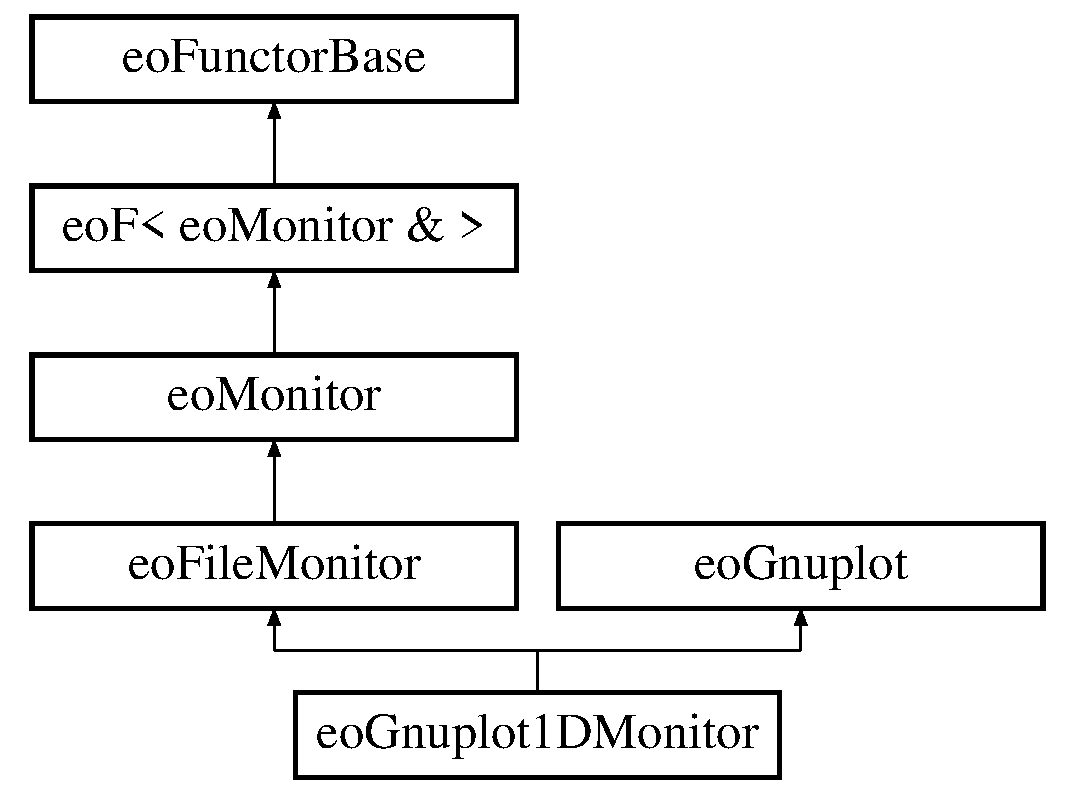
\includegraphics[height=5cm]{classeo_gnuplot1_d_monitor}
\end{center}
\end{figure}
\subsection*{Public Member Functions}
\begin{CompactItemize}
\item 
{\bf eo\-Gnuplot1DMonitor} (std::string \_\-filename, bool \_\-top=false)\label{classeo_gnuplot1_d_monitor_a0}

\begin{CompactList}\small\item\em Constructor. \item\end{CompactList}\item 
virtual {\bf $\sim$eo\-Gnuplot1DMonitor} ()\label{classeo_gnuplot1_d_monitor_a1}

\begin{CompactList}\small\item\em Destructor. \item\end{CompactList}\item 
virtual {\bf eo\-Monitor} \& {\bf operator()} ()\label{classeo_gnuplot1_d_monitor_a2}

\begin{CompactList}\small\item\em The pure virtual function that needs to be implemented by the subclass. \item\end{CompactList}\item 
virtual void {\bf First\-Plot} ()\label{classeo_gnuplot1_d_monitor_a3}

\item 
virtual std::string {\bf class\-Name} () const \label{classeo_gnuplot1_d_monitor_a4}

\begin{CompactList}\small\item\em Class name. \item\end{CompactList}\end{CompactItemize}


\subsection{Detailed Description}
Plot {\bf eo\-Stat}{\rm (p.\,\pageref{classeo_stat})}. 

\begin{Desc}
\item[Author:]Marc Schoenauer \end{Desc}
\begin{Desc}
\item[Version:]0.0 (2000)\end{Desc}
This class plots through gnuplot the {\bf eo\-Stat}{\rm (p.\,\pageref{classeo_stat})} given as argument

eo\-Gnuplot1DMonitor plots stats through gnuplot

Assumes that the same file is appened every so and so, and replots it everytime 



Definition at line 47 of file eo\-Gnuplot1DMonitor.h.

The documentation for this class was generated from the following files:\begin{CompactItemize}
\item 
eo\-Gnuplot1DMonitor.h\item 
eo\-Gnuplot1DMonitor.cpp\end{CompactItemize}
